\documentclass{classrep}
\usepackage[utf8]{inputenc}
\usepackage{graphicx}
\usepackage{listings}
\usepackage{hyperref}
\usepackage{amsmath}
\usepackage{amstext}

\studycycle{Informatyka, studia dzienne, mgr II st.}
\coursesemester{II}

\coursename{Rozpoznawanie obrazów}
\courseyear{2011/2012}

\courseteacher{dr inż. Bartłomiej Stasiak}
\coursegroup{poniedziałek, 8:15}

\author{%
  \studentinfo{Michał Janiszewski}{169485}
}

\title{Zadanie 3: zadanie problemowe.}
%\svnurl{https://serce.ics.p.lodz.pl/svn/labs/sise/mp_pt0830/jankit/genetyk}

\begin{document}
\maketitle

\section{Cel zadania}
Celem zadania było stworzenie programu, który będzie w stanie automatycznie policzyć ile na nim znajduje się winogron czerwonych i zielonych.

\section{Wprowadzenie}
Łatwo zauważyć, że winogrona mają kształt spłaszczonej kuli \ppauza na dwuwymiarowym zdjęciu ich kształt zbliżony będzie najbardziej do elipsy. Zadanie zatem sprowadza się do rozpoznania elips i oznaczenia ich jako winogrono czerwone lub czerwone. W celu odnalezienia elips wykorzystana została zmodyfikowana transformata Hougha.

\subsection{Filtr dylacji}
Dylacja to jedna z podstawowych operacji morfologicznych, stosowana najczęsciej do obrazów binarnych, której zadaniem jest powiększenie regionu obrazu zajmowanego przez pierwszy plan. Wykorzystywany jest do tego celu \textit{element strukturyzujący} (ang. \textit{structuring element}), który stanowi maskę dla operacji podobnej do splotu: jeśli w obrębie maski znajduje się w obrazie piksel zawierający pierwszy plan, to piksel będący \textit{źródłem} (ang. \textit{origin}) elementu strukturyzującego przyjmie wartość pierwszego planu; w przeciwnym przypadku piksel pozostaje pikselem tła.

\subsection{Detekcja krawędzi}
Ponieważ transformata Hougha działa na podstawie wykrytych krawędzi, istotnym celem jest zapewnienie poprawnego wykrycia krawędzi. W tym celu wykorzystane zostało różnicowe rozmycie Gaussa. Opiera się ono w skrócie o wykonanie dwóch rozmyć Gaussa dla zadanego obrazu o różnych parametrach, a następnie wyznaczenie różnic pomiędzy tymi rozmyciami.

\subsubsection{Rozmycie Gaussa}
Rozmycie Gaussa jest splotem, którego maska, o początku w punkcie $(0, 0)$, ma wartości dane wzorem:
\begin{equation}
  G(x,y) = \frac{1}{2\pi \sigma^2}e^{-\frac{x^2 + y^2}{2\sigma^2}}
\end{equation}
gdzie $\sigma$ to odchylenie standardowe.

\subsection{Detekcja elips}
W celu detekcji elips wykorzystana została zmodyfikowana transformata Hougha opisana w \cite{hough}. 

Do działania algorytm wykorzystuje następujące wzory:
\begin{equation}
\label{eq:x0}
 x_0 = (x_1 + x_2) / 2
\end{equation}
\begin{equation}
\label{eq:y0}
 y_0 = (y_1 + y_2) / 2
\end{equation}
\begin{equation}
\label{eq:a}
 a = \sqrt{(x_2 - x_1)^2 + (y_2 - y_1)^2}
\end{equation}
\begin{equation}
\label{eq:alfa}
 \alpha = \arctan{\left(\frac{x_2 - x_1}{y_2 - y_1}\right)}
\end{equation}
\begin{equation}
\label{eq:costau}
 \cos(\tau) = \frac{a^2 + d^2 - f^2}{2ad}
\end{equation}
\begin{equation}
\label{eq:b}
 b = \sqrt{\frac{a^2 d^2 \sin^2(\tau)}{a^2 - d^2\cos^2(\tau)}}
\end{equation}

\begin{figure}
  \centering
  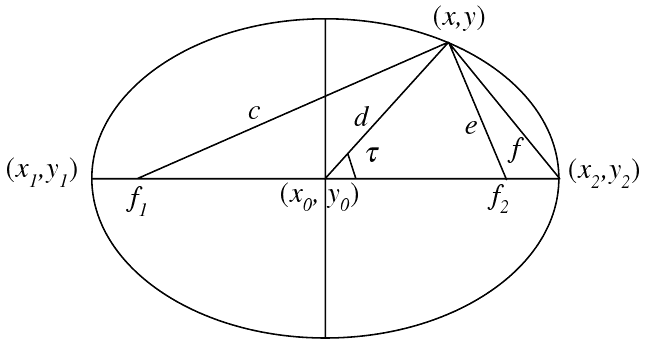
\includegraphics[width=\textwidth]{gfx/ellipse.png}
  \caption{Rysunek poglądowy elipsy}
  \label{fig:ellipse}
\end{figure}

Algorytm ma następujący przebieg:
\begin{enumerate}
  \item wszystkie piksele zawierające brzegi zapisywane są na jednej liście,
  \item akumulator jest czyszczony,
  \item dla każdego piksela $p_1 = (x_1, y_1)$ wykonywane są kroki \ref{loop1_start} do \ref{loop1_end},
  \item dla każdego innego piksela $p_2 = (x_2, y_2)$, dla którego odległość pomiędzy $p_1$, a $p_2$ jest większa niż wymagana odległość, przeprowadzane są kroki \ref{loop2_start} do \ref{loop1_end},\label{loop1_start}
  \item wykorzystując równania \ref{eq:x0}, \ref{eq:y0}, \ref{eq:a} oraz \ref{eq:alfa} obliczane są wartości $p_0 = (x_0, y_0)$, $a$ oraz $\alpha$,\label{loop2_start}
  \item dla każdego trzeciego piksela $p = (x, y)$, jeśli odległość pomiędzy $p_0$, a $p$ jest większa niż wymagana odległość, przeprowadzane są kroki \ref{loop3_start} do \ref{loop3_end},
  \item wykorzystując równania \ref{eq:costau} oraz \ref{eq:b} obliczana jest wartość $b$,\label{loop3_start}
  \item następuje zwiększenie akumulatora głosów dla danej wartości $b$,
  \item czynności są powtarzane do rozpatrzenia wszystkich pozostałych pikseli,\label{loop3_end}
  \item znajdywana jest maksymalna wartość akumulatora, jeśli przekracza ona próg wymaganych głosów, elipsa o danych parametrach zostaje oznaczona jako odnaleziona,
  \item zapisywane są parametry elipsy,
  \item piksele należące do elipsy usuwane są z tablicy wejściowej,
  \item akumulator jest czyszczony,
  \item tablica wejściowa jest przetwarzana dla wszystkich par pikseli,\label{loop1_end}
  \item koniec.
\end{enumerate}

Aby bardziej dopasować algorytm do potrzeb programu, został on dodatkowo zmodyfikowany:
\begin{itemize}
  \item znane są oczekiwane wielkości elipsy, więc głosowanie odbywa się na piksel, w którym miałoby znajdować się centrum elipsy,
  \item głosy z akumulatora sprawdzane są, czy przekraczają zadaną wartość \ppauza jeśli tak, to stwierdzone jest znalezienie elipsy,
  \item w zadanym promieniu od wykrytego centrum elipsy ilości głosów są zerowane.
\end{itemize}

\subsection{Oznaczenie koloru}
Wybór przyporządkowania wykrytej elipsy do winogron czerwonych lub zielonych odbywa się na podstawie histogramu otoczenia centrum. Piksele są przekształcane na skalę szarości a następnie poszukiwana jest część histogramu, na którą przypada większość wartości.

\section{Wyniki}
Tabela \ref{tab:results} prezentuje wyniki działania programu. $p$ jest wartością zwróconą przez program, $o$ jest wartością z ,,ręcznego'' policzenia winogron, $\delta$ to $p / o$ wyrażone w procentach.

\begin{figure}
  \begin{minipage}{0.3\linewidth}
    \centering
    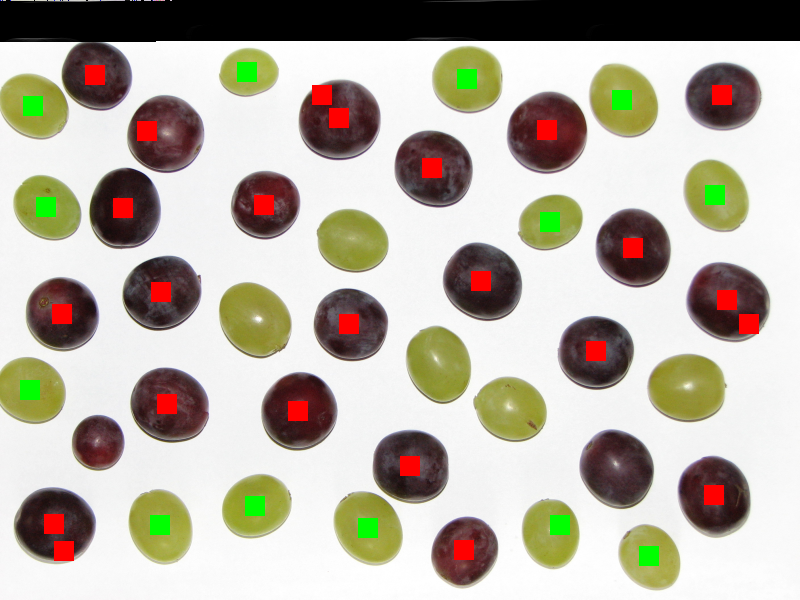
\includegraphics[width=\textwidth]{gfx/count1_overlayed.png}
    \caption{count1.png}
    \label{fig:c1}
  \end{minipage}
  \hspace{0.5cm}
  \begin{minipage}{0.3\linewidth}
    \centering
    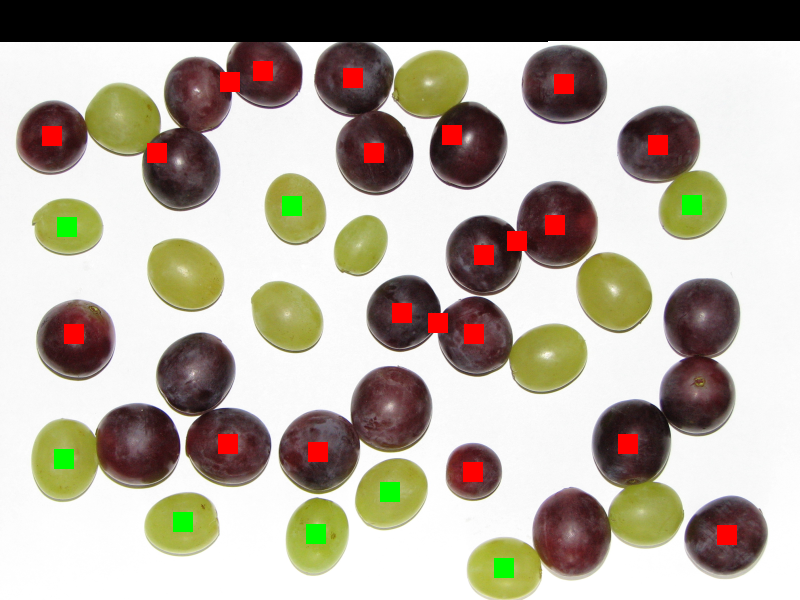
\includegraphics[width=\textwidth]{gfx/count2_overlayed.png}
    \caption{count2.png}
    \label{fig:c2}
  \end{minipage}
  \begin{minipage}{0.3\linewidth}
    \centering
    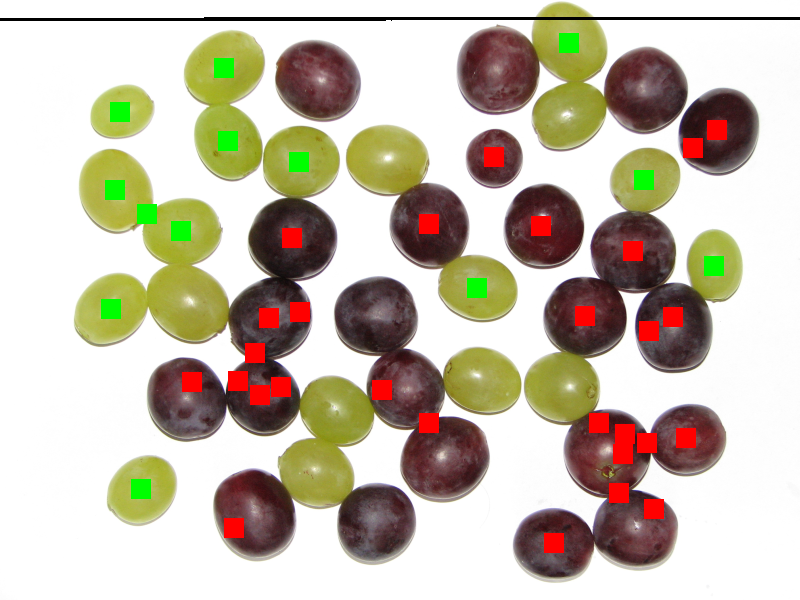
\includegraphics[width=\textwidth]{gfx/count3_overlayed.png}
    \caption{count3.png}
    \label{fig:c3}
  \end{minipage}
\end{figure}

\begin{figure}
  \begin{minipage}{0.3\linewidth}
    \centering
    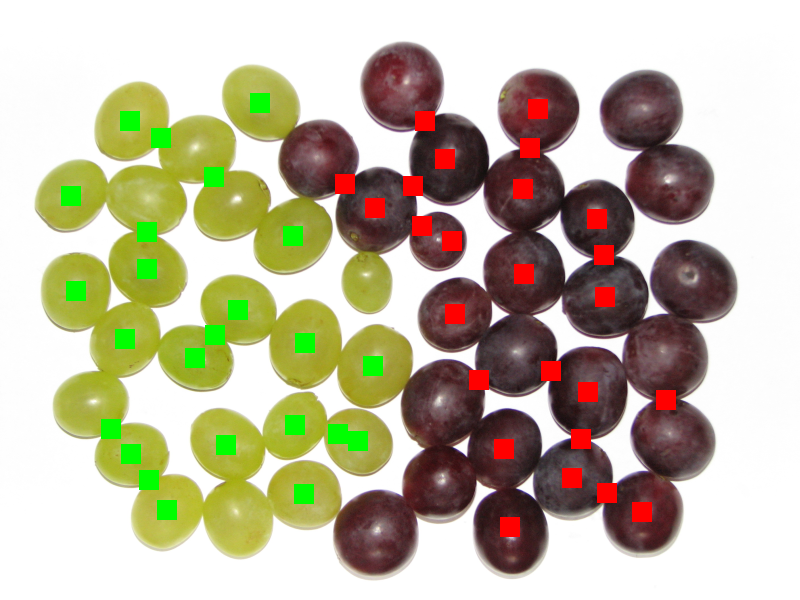
\includegraphics[width=\textwidth]{gfx/count4_overlayed.png}
    \caption{count4.png}
    \label{fig:c4}
  \end{minipage}
  \hspace{0.5cm}
  \begin{minipage}{0.3\linewidth}
    \centering
    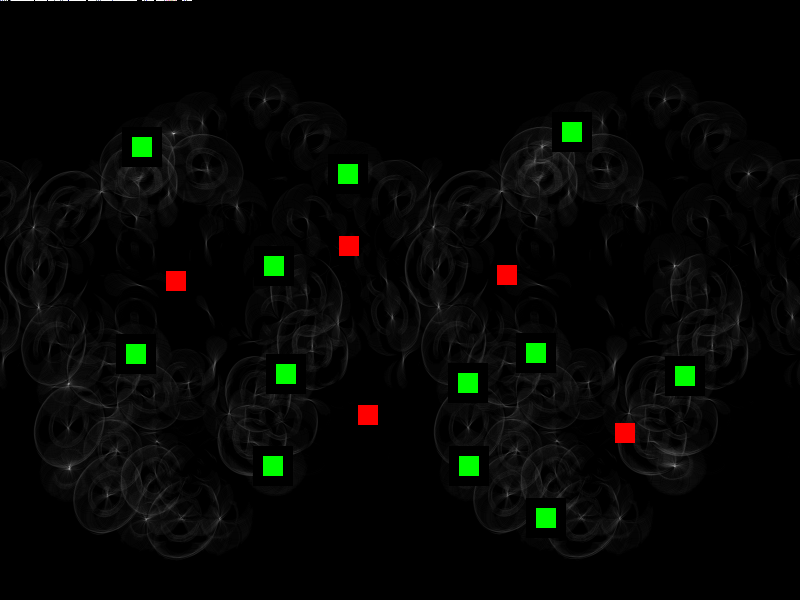
\includegraphics[width=\textwidth]{gfx/count5_overlayed.png}
    \caption{count5.png}
    \label{fig:c5}
  \end{minipage}
  \begin{minipage}{0.3\linewidth}
    \centering
    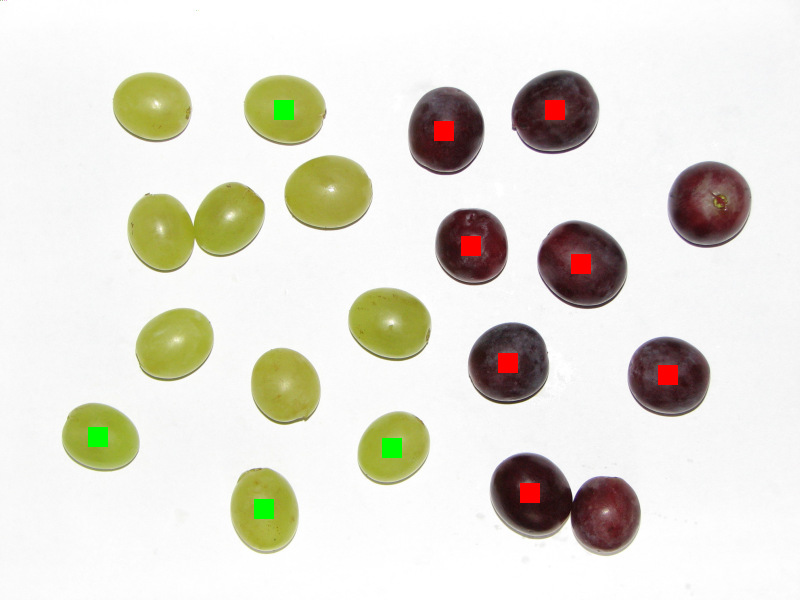
\includegraphics[width=\textwidth]{gfx/count6_overlayed.png}
    \caption{count6.png}
    \label{fig:c6}
  \end{minipage}
\end{figure}

\begin{figure}
  \begin{minipage}{0.3\linewidth}
    \centering
    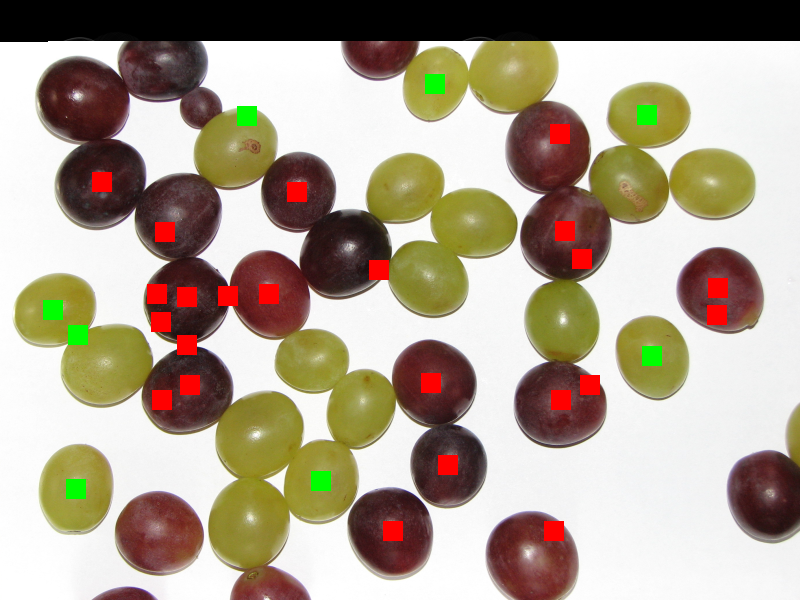
\includegraphics[width=\textwidth]{gfx/count7_overlayed.png}
    \caption{count7.png}
    \label{fig:c7}
  \end{minipage}
  \hspace{0.5cm}
  \begin{minipage}{0.3\linewidth}
    \centering
    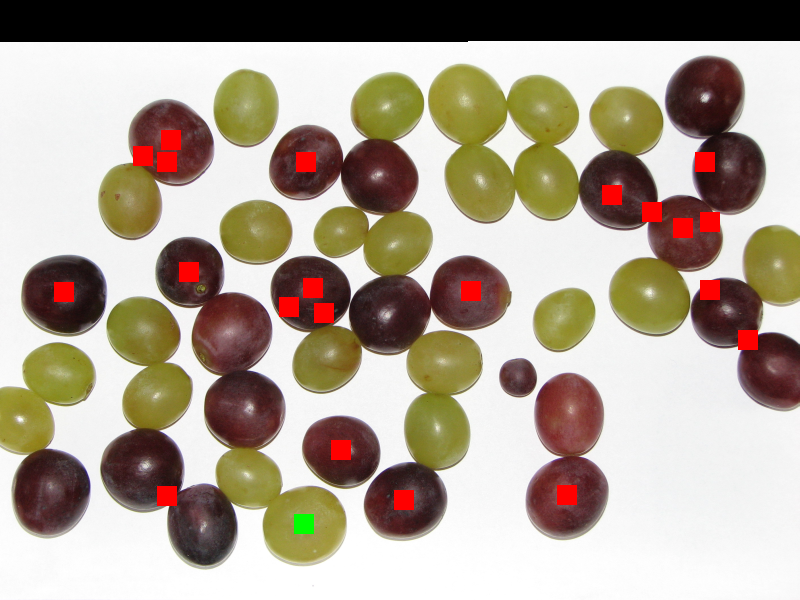
\includegraphics[width=\textwidth]{gfx/count8_overlayed.png}
    \caption{count8.png}
    \label{fig:c8}
  \end{minipage}
  \begin{minipage}{0.3\linewidth}
    \centering
    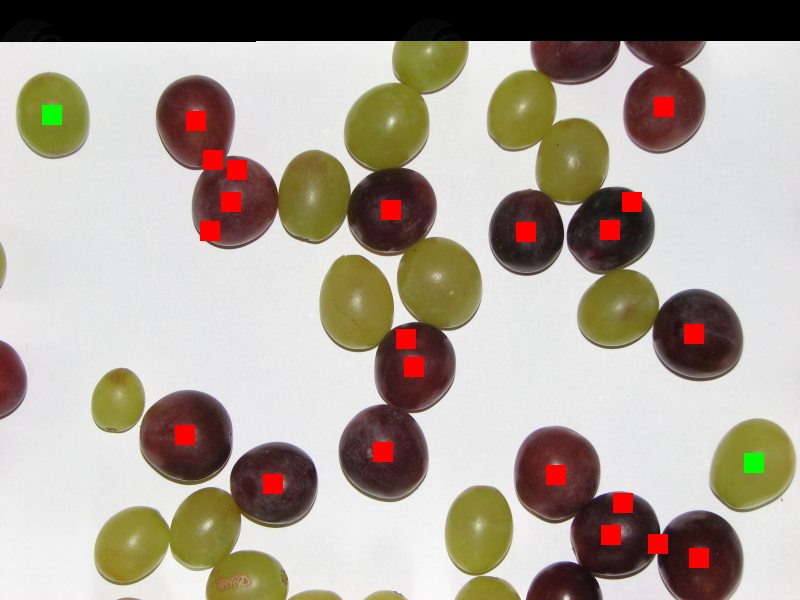
\includegraphics[width=\textwidth]{gfx/count9_overlayed.png}
    \caption{count9.png}
    \label{fig:c9}
  \end{minipage}
\end{figure}

\begin{figure}
  \begin{minipage}{0.3\linewidth}
    \centering
    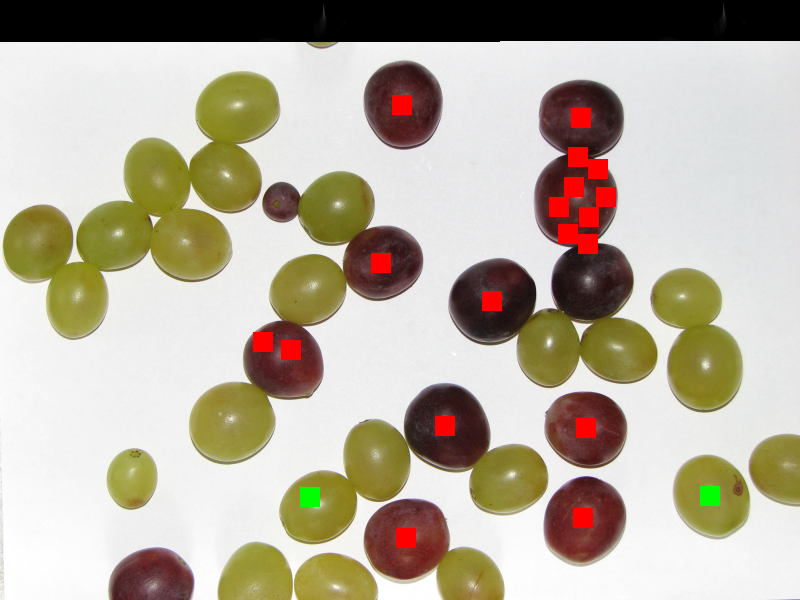
\includegraphics[width=\textwidth]{gfx/count10_overlayed.png}
    \caption{count10.png}
    \label{fig:c10}
  \end{minipage}
  \hspace{0.5cm}
  \begin{minipage}{0.3\linewidth}
    \centering
    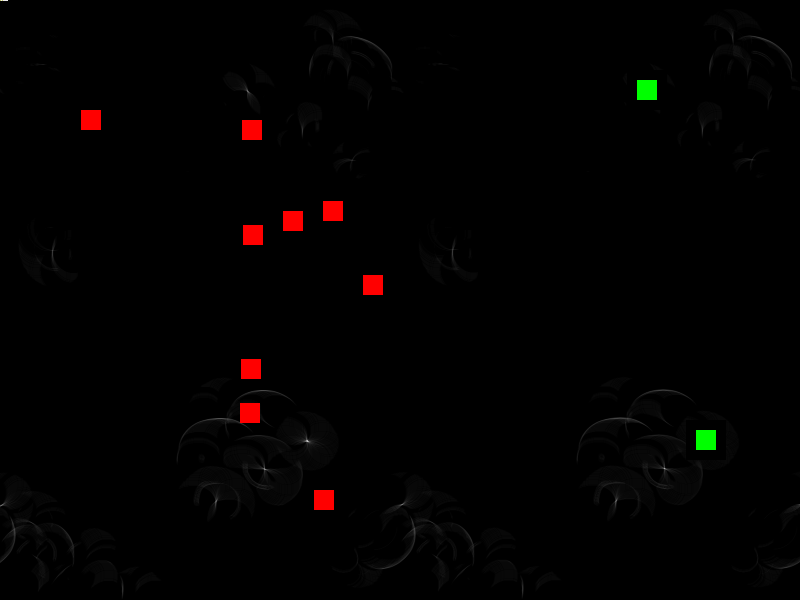
\includegraphics[width=\textwidth]{gfx/count11_overlayed.png}
    \caption{count11.png}
    \label{fig:c11}
  \end{minipage}
  \begin{minipage}{0.3\linewidth}
    \centering
    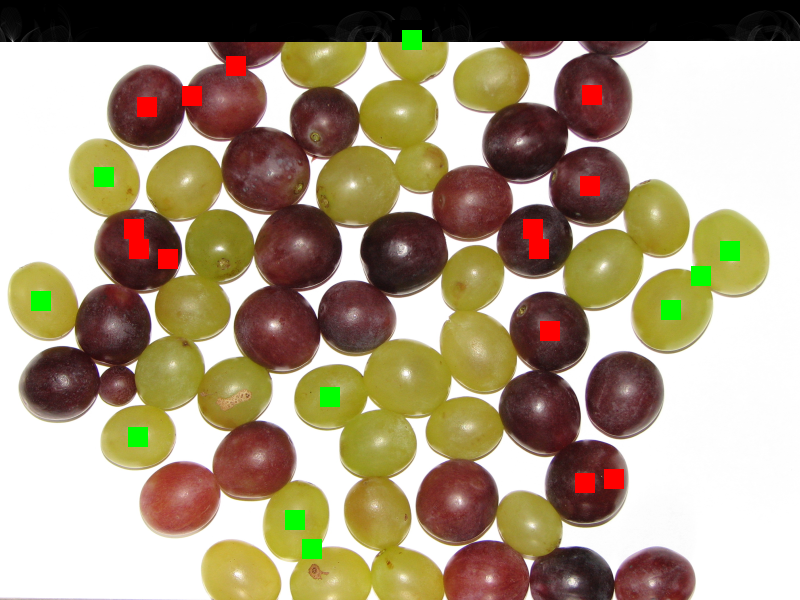
\includegraphics[width=\textwidth]{gfx/count12_overlayed.png}
    \caption{count12.png}
    \label{fig:c12}
  \end{minipage}
\end{figure}

\begin{figure}
  \begin{minipage}{0.3\linewidth}
    \centering
    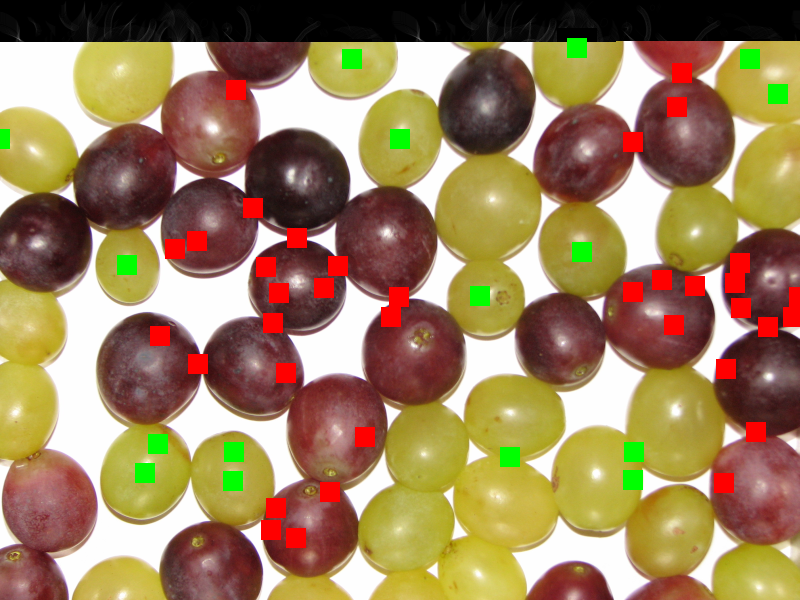
\includegraphics[width=\textwidth]{gfx/count13_overlayed.png}
    \caption{count13.png}
    \label{fig:c13}
  \end{minipage}
  \hspace{0.5cm}
  \begin{minipage}{0.3\linewidth}
    \centering
    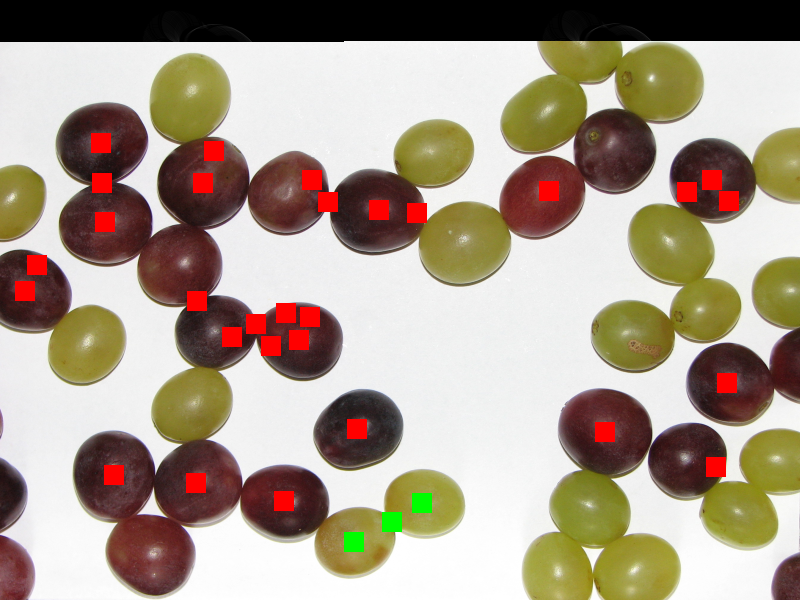
\includegraphics[width=\textwidth]{gfx/count14_overlayed.png}
    \caption{count14.png}
    \label{fig:c14}
  \end{minipage}
  \begin{minipage}{0.3\linewidth}
    \centering
    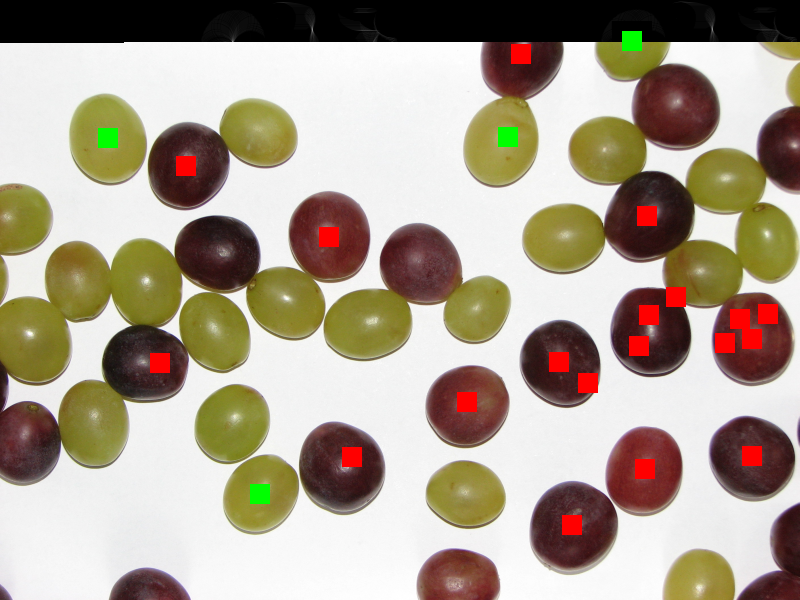
\includegraphics[width=\textwidth]{gfx/count15_overlayed.png}
    \caption{count15.png}
    \label{fig:c15}
  \end{minipage}
\end{figure}

\begin{table}
\centering
\caption{Rezultaty działania programu.}
\label{tab:results}
\begin{tabular}{|c|c|c|c|c|c|c|}
\hline
Obrazek & $o_{red}$ & $o_{green}$ & $p_{red}$ & $p_{green}$ & $\delta_{red}$ & $\delta_{green}$ \\
\hline
\hline
count01.png & 23 & 18 & 24 & 13 & 104 & 72\\
\hline
count02.png & 25 & 16 & 21 & 8 & 84 & 50\\
\hline
count03.png & 23 & 19 & 28 & 13 & 121 & 68\\
\hline
count04.png & 25 & 23 & 25 & 24 & 100 & 104\\
\hline
count05.png & 5 & 22 & 5 & 12 & 100 & 54\\
\hline
count06.png & 9 & 11 & 7 & 4 & 78 & 36\\
\hline
count07.png & 21 & 19 & 23 & 8 & 109 & 42\\
\hline
count08.png & 24 & 23 & 21 & 1 & 88 & 4\\
\hline
count09.png & 16 & 15 & 20 & 2 & 125 & 13\\
\hline
count10.png & 13 & 24 & 18 & 2 & 138 & 8\\
\hline
count11.png & 13 & 15 & 9 & 2 & 69 & 13\\
\hline
count12.png & 29 & 30 & 13 & 10 & 45 & 33\\
\hline
count13.png & 24 & 26 & 36 & 16 & 150 & 62\\
\hline
count14.png & 20 & 21 & 29 & 3 & 145 & 14\\
\hline
count15.png & 19 & 22 & 19 & 4 & 100 & 18\\
\hline
\end{tabular}
\end{table}

\section{Wnioski}
Program radzi sobie z wingronami czerwonymi znacznie lepiej niż z zielonymi. Może to wynikać z faktu, iż podczas usuwania wyników winogron czerwonych usuwane są także drobne fragmenty cieni winogron zielonych, co powoduje słabsze odnajdywanie krawędzi, a następnie problem ten propagowany jest do transformaty Hougha.

Program słabo radzi sobie z winogronami znajdującymi się na krawędzi obrazka \ppauza ich kontur nie stanowi elipsy. Aby temu zaradzić można spróbować uzależnić ilość wymaganych głosów od odległości od krawędzi, aby nie wprowadzać większej ilości fałszywych wykryć.

Program został przystosowany do dostępnych obrazków, w przypadku znacznych zmian parametrów winogron, należałoby zmiany te odwzorować w programie.

Należy także zauważyć, że wykonywanie kilkunastogodzinnych obliczeń dla obrazka o wymiarach 800$\times$600 pikseli w celu (niedokładnego) policzenia winogron nie ma absolutnie żadnego praktycznego zastosowania.

\begin{thebibliography}{0}
  \bibitem{wolfram_ellipse} Weisstein, E. W. \textit{Ellipse} w: \textit{MathWorld--A Wolfram Web Resource} [online, dostęp: 8.01.2012]. \url{http://mathworld.wolfram.com/Ellipse.html}
  \bibitem{dilation} Robert Fisher, Simon Perkins, Ashley Walker and Erik Wolfart, \textit{Morphology - Dilation} [online, dostęp 8.01.2012]. \url{http://homepages.inf.ed.ac.uk/rbf/HIPR2/dilate.htm}
  \bibitem{hough} Xie Y., Ji Q. \textit{A New Efficient Ellipse Detection Method} [online, dostęp 8.01.2012] \url{https://docs.google.com/viewer?url=www.ecse.rpi.edu/homepages/qji/Papers/ellipse_det_icpr02.pdf}
\end{thebibliography}
\end{document}

\end{document}